\documentclass[ucs, notheorems, handout]{beamer}

\usetheme[numbers,totalnumbers,minimal,nologo]{Statmod}
\usefonttheme[onlymath]{serif}
\setbeamertemplate{navigation symbols}{}
\setbeamercolor{alerted text}{fg=blue}
\usepackage{physics}

\mode<handout> {
    \usepackage{pgfpages}
    %\setbeameroption{show notes}
    %\pgfpagesuselayout{2 on 1}[a4paper, border shrink=5mm]
    \setbeamercolor{note page}{bg=white}
    \setbeamercolor{note title}{bg=gray!10}
    \setbeamercolor{note date}{fg=gray!10}
}

\usepackage[utf8x]{inputenc}
\usepackage[T2A]{fontenc}
\usepackage[english, russian]{babel}
\usepackage{tikz}
\usepackage{ragged2e}
\usepackage{graphicx}
\usepackage{subfigure}

\usepackage{amsmath}
\usepackage{amsfonts}
\usepackage{amsthm}

\DeclareMathOperator{\rk}{rk}
\DeclareMathOperator{\med}{med}
\DeclareMathOperator{\diag}{diag}
\DeclareMathOperator*{\argmin}{argmin}
\newcommand{\tX}[1]{\mathsf{#1}}

\title[Комплексные выбросы и SSA]
{Робастные варианты метода SSA для анализа комплексных временных рядов}

\subtitle
{}

\author[Сенов М.А.] 
{Сенов Михаил Андреевич}

\institute[Санкт-Петербургский Государственный Университет]{%
    \small
    Санкт-Петербургский государственный университет\\
    Прикладная математика и информатика\\
    Вычислительная стохастика и статистические модели\\
    \vspace{1.25cm}
    Отчет по научно-исследовательской работе}

\date[Зачет]{Санкт-Петербург, 2022}

\begin{document}

\begin{frame}
  \titlepage
  \note{}
\end{frame}

\begin{frame}{Введение: Проблема}

$\tX{X}_N = (x_1, \ldots, x_{N})$ временной ряд длины $N$.\\
\vspace{1em}
\alert{Модель:} $\tX{X}_N = \tX{S}_N + \tX{R}_N$, $\tX{S}_N$ сигнал, $\tX{R}_N$ шум.\\
\vspace{1em}
\alert{Проблема:} Извлечение сигнала $\tilde{\tX{S}} = F(\tX{X}_N)$, $F$ используемый метод.\\
\vspace{1em}
\alert{Метод:} SSA (Singular Spectrum Analysis) [Analysis of Time Series
Structure: SSA and Related Techniques, Golyandina N., Nekrutkin V.,
Zhigljavsky A., 2001].

    \note{}
\end{frame}

\begin{frame}{Введение: Временной ряд с выбросами и SSA}
Базовый SSA: реагирует на выбросы.
\begin{center}
    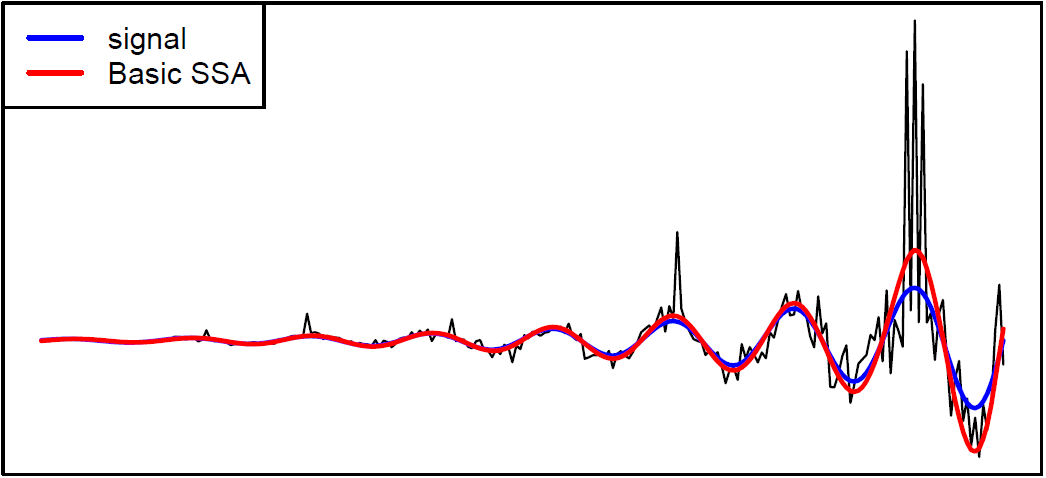
\includegraphics[, height = 3cm]{otliers_ssa.PNG}
\end{center}

Робастный SSA (Третьякова, 2020): не реагирует на выбросы.
\begin{center}
    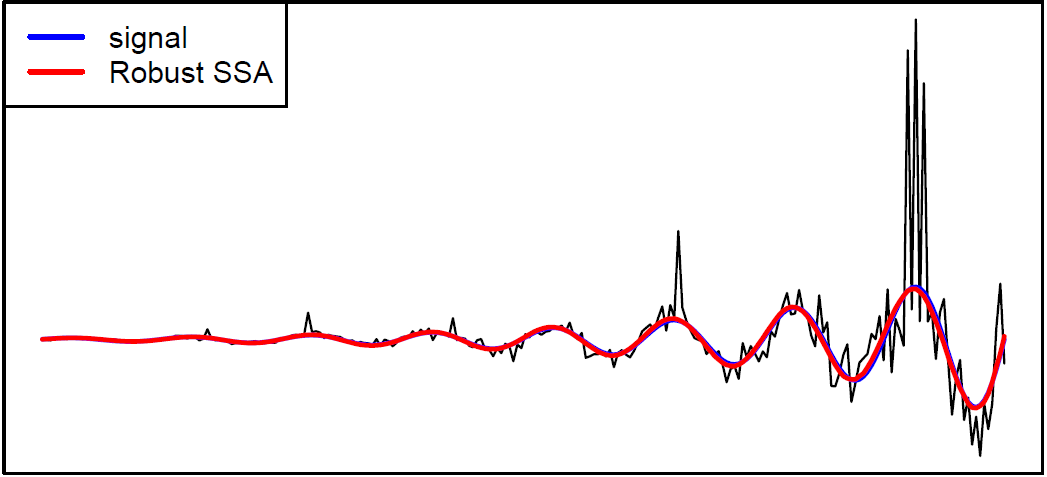
\includegraphics[, height = 3cm]{outliers_l1.PNG}
\end{center}

    \note{}
\end{frame}

\begin{frame}{Введение: Цель работы}
    Робастный SSA разработан для вещественных временных рядов.\\
    \vspace{1em}
    \alert{Цель:} Обобщить временной ряд на комплексный случай.\\
    \vspace{1em}
   Распространённый пример комплексного временного ряда~--- это инженерные задачи, где данные получаются путём преобразования Фурье.
   $$\tX{X}_N^{(t)} = (x_1^{(t)}, \ldots, x_N^{(t)}), \, t = 1 \ldots M,$$
   $$\tX{DFT}(\tX{X}_N^{(t)}) = f^{(t)}_k = \sum_{n=1}^{N}x^{(t)}_n e^{-2 \pi i k  n / N}, \, k = 1 \ldots N,$$
   $$\tX{F}^{(M)}_{k} = (f^{(1)}_k, \ldots, f^{(M)}_k).$$
\end{frame}


\begin{frame}{Методы: Определения}
Рассмотрим временной ряд $\tX{X}_N=(x_1, \ldots, x_{N})$.\\
\vspace{1em}
$\mathcal{M}_{r}$ --- пространство матриц ранга не больше $r$, размера $L \times K$,

$\mathcal{M}_{\mathcal{H}}$~--- пространство ганкелевых матриц $L\times K$.\\
\vspace{1em}
Оператор вложения $\mathcal{T}:\mathbb{R}^N \rightarrow \mathcal{M}_{\mathcal{H}}: \mathcal{T} (\tX{X_N}) = \mathbf{X} $,\\
\vspace{1em}
$\Pi_{r}:\mathcal{M}\rightarrow \mathcal{M}_r$~--- проектор на пространство матриц ранга не больше $r$ по некоторой норме в пространстве матриц,\\
\vspace{1em}
$\Pi_{\mathcal{H}}:\mathcal{M} \rightarrow \mathcal{M}_{\mathcal{H}}$~--- проектор на пространство ганкелевых матриц по некоторой норме в пространстве матриц.

    \note{}

\end{frame}

\begin{frame}{Методы: Выделение сигнала}

Временной ряд $\tX{X}_N=(x_1, \ldots, x_{N})$.
\begin{block}{Алгоритм для выделения сигнала}
\begin{equation*}
	\tilde{\tX{S}} = \mathcal{T}^{-1} \Pi_{\mathcal{H}} \Pi_{r} \mathcal{T} (\tX{X_N}).
\end{equation*}
\end{block}


Нормы для $\Pi_r$ и $\Pi_{\mathcal{H}}$:
\begin{itemize}
        \item $\mathbb{L}_2$(Фробениус): выделение сигнала базовым SSA.
        \item $\mathbb{L}_1$: робастная версия SSA.
        \item weighted $\mathbb{L}_2$ (присвоение веса каждому элементу): робастная версия SSA.
\end{itemize}
    \note{}
\end{frame}


\begin{frame}{Методы: Иллюстрирующий пример}
    \begin{block}{Пример}
    $(x_1, \ldots, x_N)$, норма $p(x)$, $\argmin\limits_{c}p((x_1 - c, \ldots, x_N - c)) =\, ?$
    \end{block}
    Нормы:
    \begin{itemize}
        \item $\mathbb{L}_2$. $\overline{x} = \argmin\limits_{c} \sqrt{\sum_{i = 1}^{N} |x_i - c|^2}$. \\
        Если $x_i \to \infty$, тогда $\overline{x} \to \infty$. Не робастный.
        \item $\mathbb{L}_1$. $\med = \argmin\limits_{c} \sum_{i = 1}^{N} |x_i - c|$. \\
        Если $x_i \to \infty$, тогда $\med \not\to \infty$. Робастный.
        \item weighted $\mathbb{L}_2$. $\overline{x}_w = \argmin\limits_{c} \sqrt{\sum_{i = 1}^{N} w_i|x_i - c|^2}$.\\
        Если $x_i \rightarrow \infty$, тогда возьмём $w_i = 0$ и $\overline{x}_w \not\to \infty$. Робастный.
    \end{itemize}
\end{frame}

\begin{frame}{CSSA ($\mathbb{L}_2$)}
    Траекторная матрица $\mathbf{Y} \in \mathbb{C}^{L\times K}$ на вход.\\
    
    \begin{block}{Задача}
    \begin{equation*}
	    \|\mathbf{Y}-\mathbf{M}\mathbf{V}^{\mathrm{H}}\|_F^2 \longrightarrow \min_{\mathbf{M},\mathbf{V}}, \, \mathbf{M} \in \mathbb{C}^{L\times r}, \mathbf{V} \in \mathbb{C}^{K\times r}
    \end{equation*}
    \end{block}
    $$\tX{SVD}(\mathbf{Y}) = \sum_{i = 1}^{r} \sqrt{\lambda_i}U_i V_i^{\mathrm{H}} = \mathbf{U} \mathbf{\Lambda} \mathbf{V}^{\mathrm{H}},$$
    $U_i$ собственный вектор $\mathbf{Y} \mathbf{Y}^{\mathrm{H}}$, $\lambda_i$ $i$-ое  собственное число $\mathbf{Y} \mathbf{Y}^{\mathrm{H}}$, $V_i$~собственный вектор $\mathbf{Y}^{\mathrm{H}} \mathbf{Y}$.\\
    \vspace{1em}
    Точное решение $\mathbf{M}\mathbf{V}^{\mathrm{H}}$, $\mathbf{M} = \mathbf{U} \mathbf{\Lambda}$.

    \note{}
\end{frame}

\begin{frame}{$\mathbb{L}_1$}

Траекторная матрица $\mathbf{Y} \in \mathbb{C}^{L\times K}$ на вход.
\begin{block}{Задача}
\begin{equation*}
	\|\mathbf{Y}-\mathbf{M}\mathbf{V}^{\mathrm{H}}\|_1 \longrightarrow \min_{\mathbf{M},\mathbf{V}}, \, \mathbf{M} \in \mathbb{C}^{L\times r}, \mathbf{V} \in \mathbb{C}^{K\times r}
\end{equation*}
\end{block}
Точного решения нет. Решаем итеративно 
\begin{equation*}
	 \mathbf{M(t)} = \argmin\limits_{\mathbf{M}\in \mathbb{C}^{L\times r}} \|\mathbf{Y} - \mathbf{M}\mathbf{V}^\mathrm{H}(t - 1)\|_1
\end{equation*}
$$\mathbf{V(t)} = \argmin\limits_{\mathbf{V}\in \mathbb{C}^{K\times r}} \|\mathbf{Y} - \mathbf{M}(t)\mathbf{V}^\mathrm{H}\|_1.$$

Может быть сведено к линейному случаю и решено при помощи нахождения взвешенной медианы.
    \note{}
\end{frame}


\begin{frame}{Weighted $\mathbb{L}_2$: Алгоритм}

Траекторная матрицы $\mathbf{Y} \in \mathbb{C}^{L\times K}$ на вход.\\ 
\vspace{1em}
Итеративно вычисляем матрицу весов $\mathbf{W} \in \mathbb{R}^{L\times K}$ .
\begin{block}{Задача}
\begin{equation*}
	\|\mathbf{W}^{1/2}\odot(\mathbf{Y}-\mathbf{M}\mathbf{V}^{\mathrm{H}})\|^{2}_F \longrightarrow \min_{\mathbf{M},\mathbf{V}}, \, \mathbf{U} \in \mathbb{C}^{L\times r}, \mathbf{V} \in \mathbb{C}^{K\times r}
\end{equation*}
\end{block}
Точного решения нет. Решаем итеративно
\begin{equation*}
	\mathbf{M(t)} = \argmin\limits_{\mathbf{M}\in \mathbb{C}^{L\times r}} \|\mathbf{W}^{1/2}\odot(\mathbf{Y}-\mathbf{M}\mathbf{V}^{\mathrm{H}}(t-1))\|^2_F
\end{equation*}
$$\mathbf{V(t)} = \argmin\limits_{\mathbf{V}\in \mathbb{C}^{K\times r}} \|\mathbf{W}^{1/2}\odot(\mathbf{Y}-\mathbf{M}(t)\mathbf{V}^{\mathrm{H}})\|^2_F$$
Может быть сведено к IRLS.

    \note{}
\end{frame}

% \begin{frame}{Методы: Проблемы}
%     Траекторная матрица $\mathbf{Y} \in \mathbb{C}^{L\times K}$ на вход.\\ 
%     Обозначим $\mathbf{M} \in \mathbb{C}^{L\times r}, \mathbf{V} \in \mathbb{C}^{K\times r}, \mathbf{W} \in \mathbb{R}^{L\times K}$.\\
%     \vspace{1em}
%     Методы решают следующие проблемы:
%     \begin{itemize}
%         \item $\mathbb{L}_2$ CSSA: 
%         $$ \|\mathbf{Y}-\mathbf{M}\mathbf{V}^{\mathrm{H}}\|_F^2 \longrightarrow \min_{\mathbf{M},\mathbf{V}},$$
%         имеет точное решение.
%         \item $\mathbb{L}_1$ CSSA:
%         $$\|\mathbf{Y}-\mathbf{M}\mathbf{V}^{\mathrm{H}}\|_1 \longrightarrow \min_{\mathbf{M},\mathbf{V}}.$$
%         решение вычисляется итеративно.
%         \item weighted $\mathbb{L}_2$ CSSA:
%         $$\|\mathbf{W}^{1/2}\odot(\mathbf{Y}-\mathbf{M}\mathbf{V}^{\mathrm{H}})\|^{2}_F \longrightarrow \min_{\mathbf{M},\mathbf{V}},$$
%         решение вычисляется итеративно, $\mathbf{W}$ обновляется на каждой итерации. 
%     \end{itemize}
% \end{frame}

\begin{frame}{Weighted $\mathbb{L}_2$: Вычисление весов}
Выброс определяется по абсолютному значению.
    \begin{block}{Алгоритм}
    \begin{enumerate}
        \item Вычисление матрицы остатков $\mathbf{R} = \{r_{ij}\}_{i,j=1}^{n,p} = \mathbf{Y} - \mathbf{M}\mathbf{V}^\mathrm{H}$
        \item Обновление матрицы $\mathbf{\Sigma} =      \{\sigma_{ij}\}^{L,K}_{i,j=1}$
        \item Вычисление весов $\mathbf{W} = \{w_{ij}\}^{L,K}_{i,j=1} = \{w(\frac{r_{ij}}{\sigma_{ij}})\}^{L,K}_{i,j=1}$, используя
        $$w(x) = 
        \begin{cases}
        (1 - (\frac{|x|}{\alpha})^2)^2 &|x| \leq \alpha\\
        0 &|x| > \alpha\\
        \end{cases}$$
    \end{enumerate}    
    \end{block}
    Алгоритм аналогичен методу LOESS (aka LOWESS).
    \note{}
\end{frame}

\begin{frame}{Weighted $\mathbb{L}_2$: Гетероскедастичный шум}
     Рассмотрим временной ряд с гетероскедастичным шумом.
     \begin{center}
        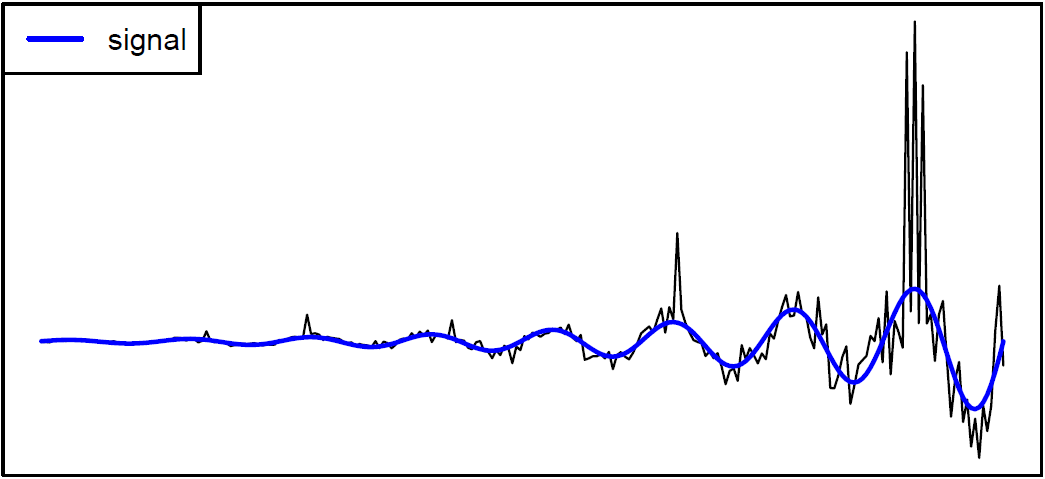
\includegraphics[, height = 3cm]{signal.PNG}
    \end{center}
     Правосторонние элементы, не являющиеся выбросами, больше чем левосторонние выбросы.\\
     \vspace{1em}
     \alert{Базовый:} Нормализующие коэффициенты $\sigma_{ij}$ одинаковы для каждого элемента ряда. Выявление выбросов некорректно.\\
     \vspace{1em}
     \alert{Модификация:} Вычислять $\sigma_{ij}$ как тренд ряда остатков.
\end{frame}

\begin{frame}{Вещественные выбросы: Временной ряд}
    Мотивация:
    \begin{itemize}
        \item Рассмотреть специфичный случай неравномерного распределения выбросов по вещественной и мнимой осям.
    \end{itemize}
    \vspace{1em}
    \alert{Пример}:
    Временной ряд длины $N = 240$,
    $$f_n = e^{4n/N} e^{2n\pi/30i},$$
    с $5\%$ выбросов и значением выброса $5\Re(f_i)$.
    \begin{figure}[ht]
    \subfigure[Re]{
    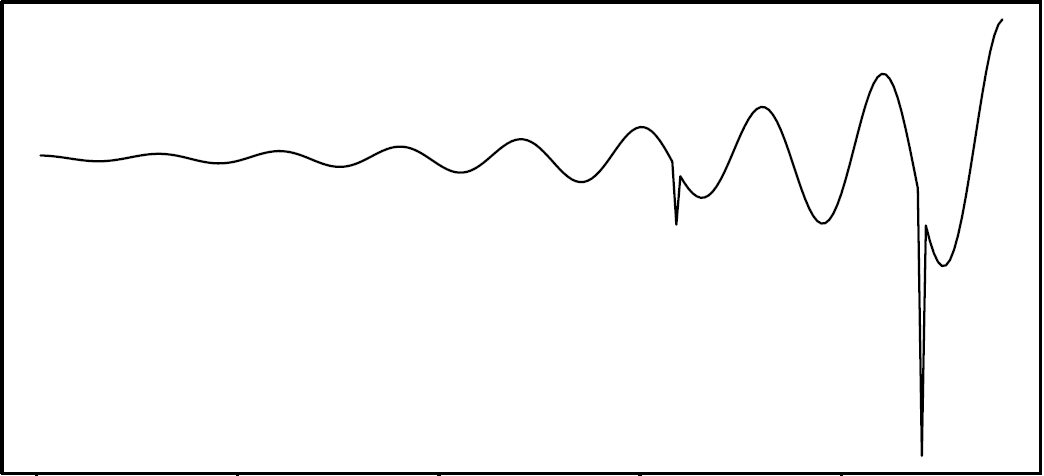
\includegraphics[, height = 2cm]{Re_outl_Re.PNG}
    }
    \subfigure[Im]{
    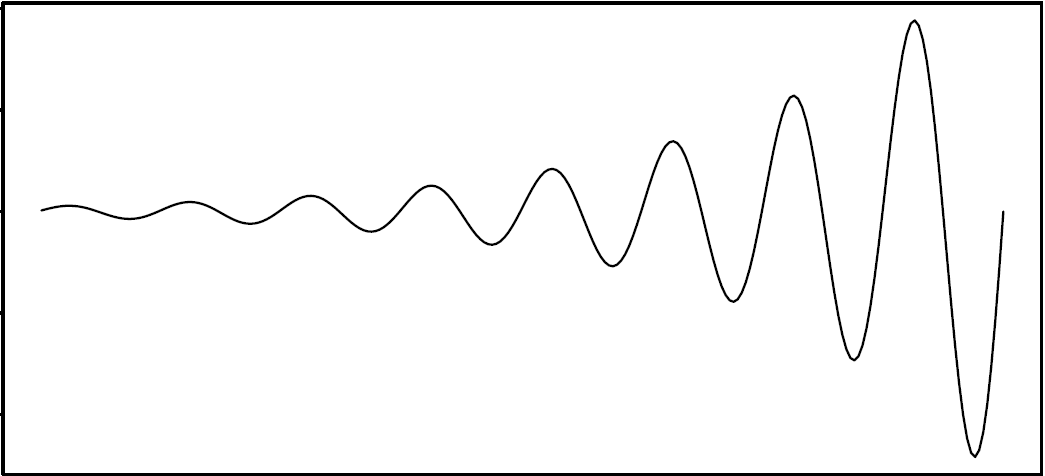
\includegraphics[, height = 2cm]{Re_outl_Im.PNG}
    }
    \end{figure}
\end{frame}

\begin{frame}{Вещественные выбросы: Модификация}
    \alert{База:} $w(x)$ зависит от $|x|$.\\
    \alert{Модификация:} $w(x)$ зависит от $|\Re(x)|$.\\
    \vspace{1em}
    Сравним результаты:
    \begin{table}[H]
	\begin{center}
		\caption{сравнения RMSE}
		\label{tab3}
		\begin{tabular}{|c|c|c|c|}
			\hline
			Ряд & w-L2 abs & w-L2 Re & p-value \\ 
			\hline
			complex & 0.053  & 0.053 & 0.62 \\
			\hline
			Re & 0.037  & 0.037 & 0.56 \\
			\hline
			Im & 0.38  & 0.038 & 0.69 \\
			\hline
		\end{tabular}
	\end{center}
    \end{table}
    p-value для t-test с зависимой выборкой из $30$ наблюдений.\\
    \vspace{1em}
    Модификация не даёт отличий по ошибке ни в одном из случаев.
\end{frame}

\begin{frame}{Вещественные выбросы: Ошибка восстановления}
    Посмотрим на остатки восстановления для CSSA (SVD).
   \begin{figure}[ht]
    \subfigure[Re]{
    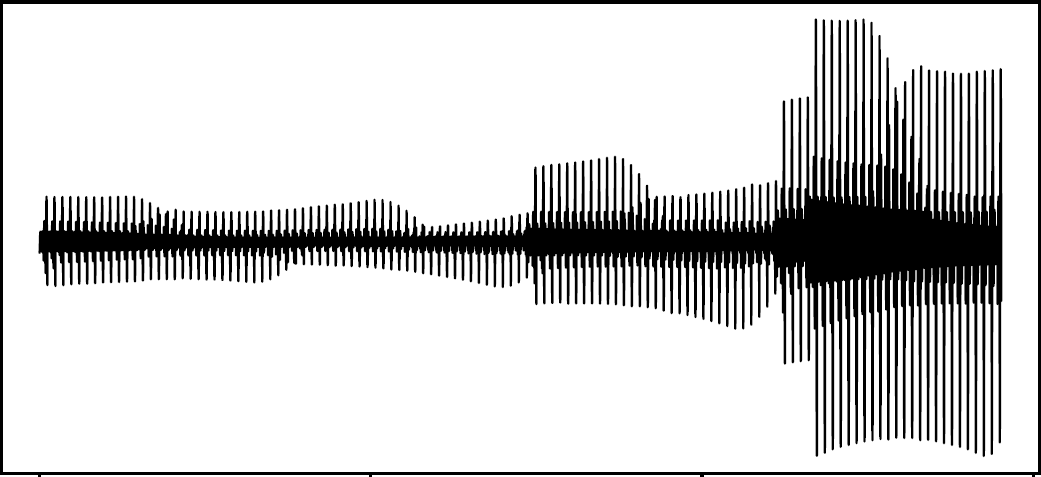
\includegraphics[, height = 2.3cm]{Res_Re.PNG}
    }
    \subfigure[Im]{
    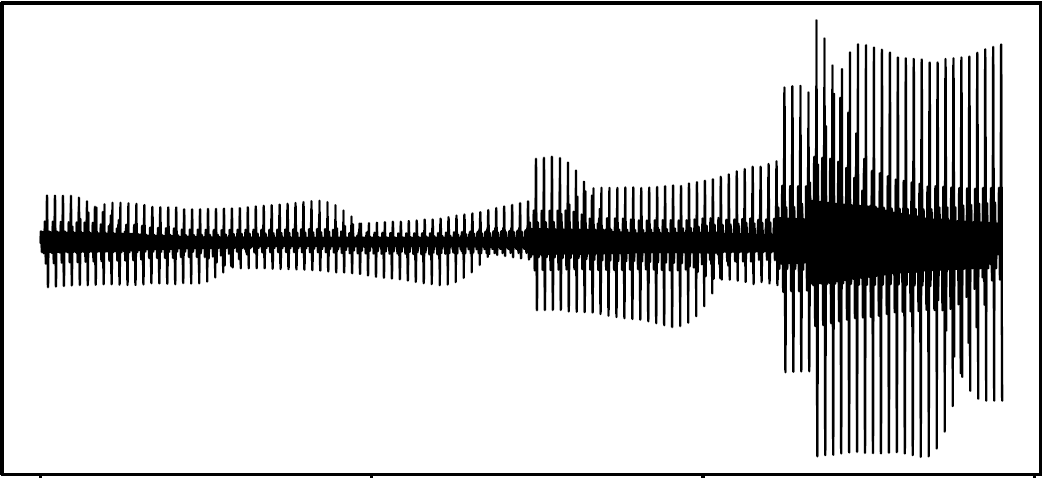
\includegraphics[, height = 2.3cm]{Res_Im.PNG}
    }
    \caption{ряд из матрицы остатков}
    \end{figure}
    \alert{Вывод:} Местоположение выбросов не влияет на ошибку восстановления.
\end{frame}
\begin{frame}{Ошибка восстановления: Определения}
    \alert{Модель:} $S(\delta) = S + \delta R$ длины $N$\\
    или\\
     $\mathbf{H}(\delta) = \mathbf{H} + \delta \mathbf{E}$, где $\mathbf{H}(\delta) = \mathcal{T}(S(\delta))$, $\mathbf{H} = \mathcal{T}(S)$, $\delta\mathbf{E} = \mathcal{T}(\delta R)$ для длины окна $L$.\\
     $\mathbf{P}_k$~--- проектор на $k$-ое ортогональное собственное пространство $\mathbf{H}\mathbf{H}^{\mathrm{H}}$.\\
     $\mathbf{P}_k(\delta) = \mathbf{P}_k + \delta\mathbf{P}^{(1)}_k +  \delta^2\mathbf{P}^{(2)}_k + \ldots$\\
     $\mathbf{H}_k(\delta) = \mathbf{P}_k(\delta) \mathbf{H} = \mathbf{H}_k + \delta\mathbf{H}^{(1)}_k +  \delta^2\mathbf{H}^{(2)}_k + \ldots$\\
     \vspace{1em}
     $\mathbf{H}^{(1)} = \sum_{i = 1}^{r} \mathbf{H}^{(1)}_i$\\
     $f^{(1)} = \mathcal{H}(\mathbf{H}^{(1)})$ первый порядок ошибки восстановления.\\
     \vspace{1em}
     При $\rk \mathbf{H} \leq 2$ известны формулы для $\mathbf{H}^{(1)}$ через сингулярные вектора в вещественном случае (Некруткин, 2008).
\end{frame}

\begin{frame}{Ошибка восстановления: Формулы для $\mathbf{H}^{(1)}$}
Комплексное обобщение формул для $\mathbf{H}^{(1)}$.\\
\vspace{1em}
Для $\rk S = 2$ и сингулярных векторов $U_1$, $U_2$, $V_1$, $V_2$ матрицы $\mathbf{H} \mathbf{H}^{\mathrm{H}}$
    \begin{multline*}
\mathbf{H}^{(1)}(\mathbf{E}, S) = U_1 U^{\mathrm{H}}_1 \mathbf{E} + U_2 U^{\mathrm{H}}_2 \mathbf{E} + \mathbf{E} V_1 V^{\mathrm{H}}_1 + \mathbf{E} V_2 V^{\mathrm{H}}_2 -
 \\
 -(\alpha_{11} U_1 V^{\mathrm{H}}_1 + \alpha_{12} U_1 V^{\mathrm{H}}_2 + \alpha_{21} U_2 V^{\mathrm{H}}_1 + \alpha_{22} U_2 V^{\mathrm{H}}_2)
\end{multline*}
где $\alpha_{ij} = U_i \mathbf{E} V^{\mathrm{H}}_j$.\\
\vspace{1em}
Для $\rk S = 1$ и сингулярных векторов $U_1$, $V_1$ 

\begin{equation*}
	\mathbf{H}^{(1)}(\mathbf{E}, S) = -U_1^{\mathrm{H}} \mathbf{E} V_1 U_1 V^{\mathrm{H}}_1 + U_1 U^{\mathrm{H}}_1 \mathbf{E} + \mathbf{E} V_1 V^{\mathrm{H}}_1
\end{equation*}
\end{frame}

\begin{frame}{Ошибка восстановления: Теорема}
    $f^{(1)} = \mathcal{H}(\mathbf{H}^{(1)}(\mathbf{E}, S))$

    $f^{(1)*}_{\Re} = \mathcal{H}(\mathbf{H}^{(1)}(\mathbf{\Re(E)}, \Re(S)))$ 

    $f^{(1)*}_{\Im} = \mathcal{H}(\mathbf{H}^{(1)}(\mathbf{\Im(E)}, \Im(S)))$
    
    \begin{block}{Теорема \label{th:sum}}
        Пусть сингулярные вектора $S$, $\Re(S)$ и $\Im(S)$ совпадают и $\rk S \leq 2$.
	
	Тогда $$f^{(1)} = f^{(1)*}_{\Re(S)} + if^{(1)*}_{\Im(S)}.$$
    \end{block}
    
	Примером сигнала, для которого в общем случае очевидно не выполняются требования теоремы, является комплексная экспонента $s_n = e^{\phi(n) + i\psi(n)}$, поскольку $\rk S = 1$, а $\rk\Re(S) = \rk\Im(S) = 2$.

\end{frame}

\begin{frame}{Шум: Дисперсия ошибки}
    $R$~--- шум, $\Re(R)$ и $\Im(R)$ независимы.\\
    \vspace{1em}
    \alert{Известно:} Пусть $\zeta = \xi + i\eta$, $\ksi$ и $\eta$ независимы. Тогда $\mathbb{D}(\zeta) = \mathbb{D}(\xi) + \mathbb{D}(\eta)$.
    \begin{block}{Утверждение}
        Пусть выполнены условия теоремы.
	
	Тогда
	\begin{equation} \label{eq:dispsum}
	\mathbb{D}f^{(1)}_l = \mathbb{D}f^{(1)*}_{\Re, l} + \mathbb{D}f^{(1)*}_{\Im, l}.	
	\end{equation}
    \end{block}
    
    В случае $\rk S = 2$, численными экспериментами показано, что равенство \eqref{eq:dispsum} приближённо выполнено для синусоидальных сигналов со сдвигом, не равным $\pi / 2$  (Golyandina~et~al.,~SSA~with~R).
\end{frame}

\begin{frame}{Шум: Частный случай}
    Рассмотрим сигнал с $s_n = c_1 + ic_2$ и матрицу шума $\mathbf{E}$ с  $\mathbb{D}\Re(\mathbf{E}_{ij}) = \sigma_1$ и $\mathbb{D}\Im(\mathbf{E}_{ij}) = \sigma_2$.\\
    \vspace{1em}
    $\Re(S) = c_1$, $\Im(S) = c_2$.\\
    \vspace{1em}
    Для рядов c $S = c$ и белым шумом известна формула дисперсии для каждого элемента ошибки (Власьева, 2008).\\
    \vspace{1em}
    Тогда, по утверждению: $\mathbb{D} f^{(1)}_l = \mathbb{D} f^{(1)*}_{\Re, l} + \mathbb{D} f^{(1)*}_{\Im, l}$,\\
    где формулы для $\mathbb{D} f^{(1)*}_{\Re, l}$ и $\mathbb{D} f^{(1)*}_{\Im, l}$ известны.
\end{frame}

\begin{frame}{Выбросы: Матрица ошибки}
    Рассматриваем ряд с $S = c_1 + ic_2$ и выбросом $a + ib$ на позиции $k$.\\
    По теореме достаточно рассматривать ряд с вещественным выбросом $a$ на позиции $k$.\\
    \vspace{1em}
    Не умаляя общности предполагаем, что $L \leq K = N - L + 1$\\
    \vspace{1em}
    Для $1 \leq k < L$
    $$\mathbf{H}^{(1)} = \frac{a}{LK}\begin{pmatrix}
	(L + K - k) & \ldots & (L + K - k) & \ldots & (L - k)\\
	\vdots & & \vdots & & \vdots \\
	(L + K - k) & \ldots & (L + K - k) & \ldots & (L - k) & \\
	\vdots & & \vdots & & \vdots \\
	(K - k) & \ldots & (K - k) & \ldots & -k \\
\end{pmatrix}$$
\end{frame}

\begin{frame}{Выбросы: Матрица ошибки}
    Для $L \leq k \leq K$
    $$\mathbf{H}^{(1)} = \frac{a}{L}\begin{pmatrix}
	0 & \ldots & 1 & \ldots & 1 & \ldots & 0\\
	\vdots & & \vdots & & \vdots & & \vdots\\
	0 & \ldots & 1 & \ldots & 1 & \ldots & 0
    \end{pmatrix}$$
    
    Для $K < k \leq N$\\
    \vspace{1em}
    Матрица выглядит как транспонированная относительно побочной диагонали $\mathbf{H}^{(1)}$ для первого случая.\\
    \vspace{1em}
\end{frame}

\begin{frame}{Выбросы: Пример}
    Формула для $f^{(1)}_l$ также была получена и представлена в работе, с численной проверкой для случая \\
    $s_n = 1 + i$, $N = 50$, $L = 20$, $a = 10$, $k = 3$.
    \begin{figure}[H]    
     \begin{center}
        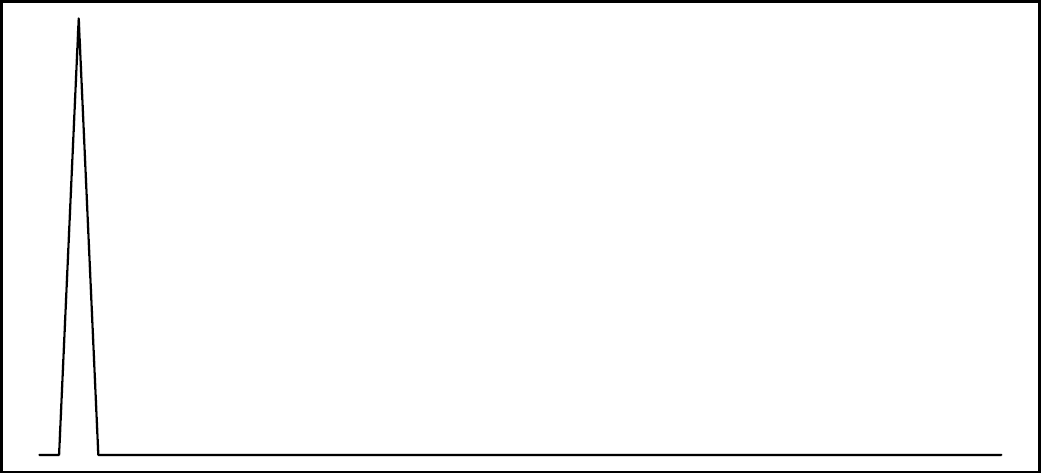
\includegraphics[, height = 2.2cm]{F_outl.PNG}
        \caption{График вещ. части ряда с выбросом.}
    \end{center}
\end{figure}
\begin{figure}[H]    
     \begin{center}
        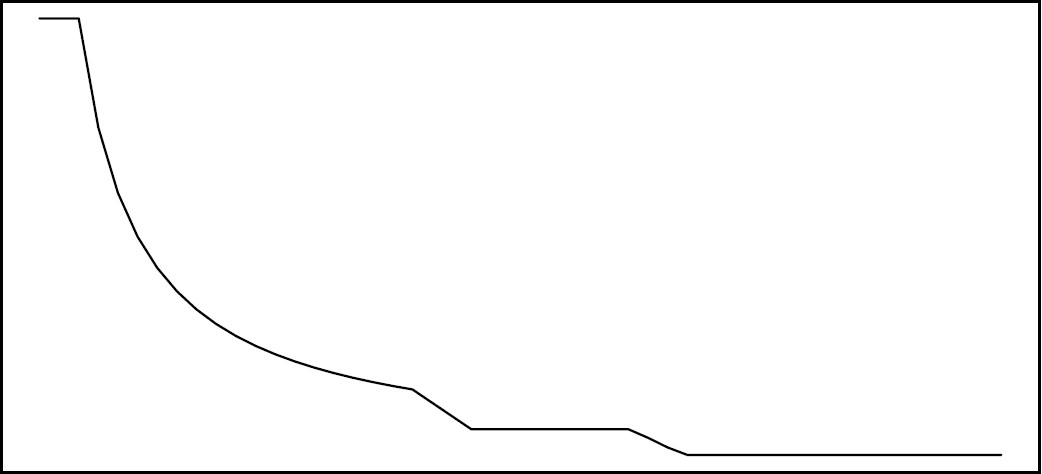
\includegraphics[, height = 2.2cm]{f1_outl.PNG}
        \caption{График $\Re(f^{(1)})$.}
    \end{center}
\end{figure}
\end{frame}


\begin{frame}{Выбросы: свойство сохранения RMSE}
    \alert{Обозначение:} $RMSE = \sqrt{\frac{1}{N}\sum_{l = 1}^{N} (f^{(1)}_l)^2}$ для ряда $F = S + R$
    \begin{block}{Утверждение}
        Пусть сигнал $S$ удовлетворяет условиям теоремы. \\
	\vspace{1em}
	Тогда RMSE для ряда с сигналом $S$ и выбросом $a + ib$, и  ряда с сигналом $S$ и выбросом $a^* + ib^*$, таким что $|a^* + ib^*| = |a + ib|$, совпадают.
    \end{block}
\end{frame}

\begin{frame}{Комплексная экспонента: Временной ряд}
    Мотивация:
    \begin{itemize}
        \item Для комплексной экспоненты не выполняются условия теоремы, хотим проверить на примере, применим ли её результат.
    \end{itemize}
    \vspace{1em}
    \alert{Пример}:
    Временной ряд длины $N = 240$,
    $$f_n = e^{4n/N} e^{2n\pi/30i},$$
    с $5\%$ выбросов и значением выброса $5\Re(f_i)$.
    \begin{figure}[ht]
    \subfigure[Re]{
    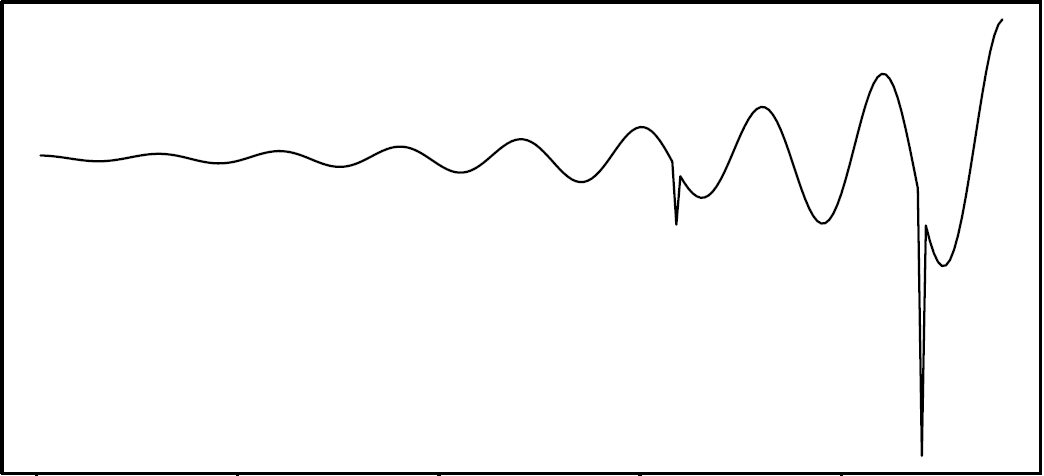
\includegraphics[, height = 2cm]{Re_outl_Re.PNG}
    }
    \subfigure[Im]{
    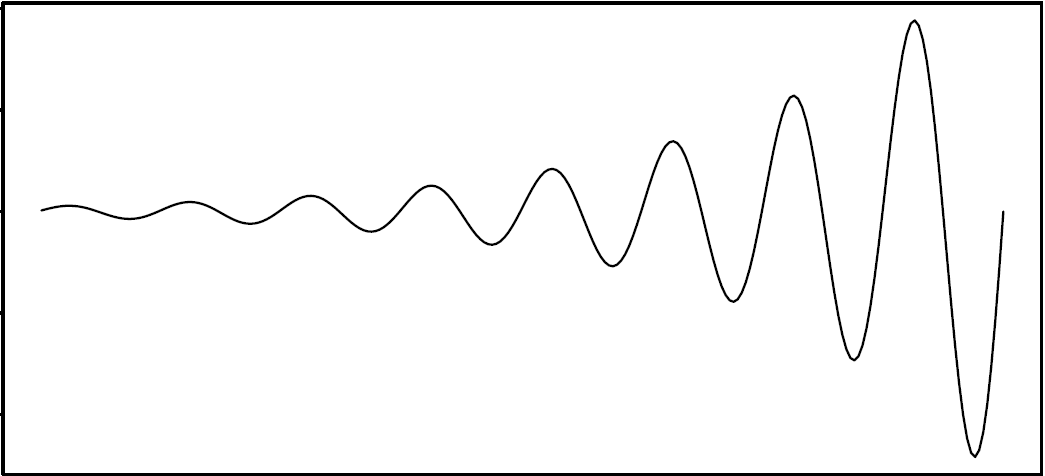
\includegraphics[, height = 2cm]{Re_outl_Im.PNG}
    }
    \end{figure}
\end{frame}

\begin{frame}{Комплексная экспонента: Сравнение}
    Рассмотрим $\Re(f^{(1)})$ и $\Im(f^{(1)})$, проверим, ведут ли они себя так же, как $f^{(1)*}_{\Re}$ и $f^{(1)*}_{\Im}$.

\begin{figure}[H]    
     \begin{center}
        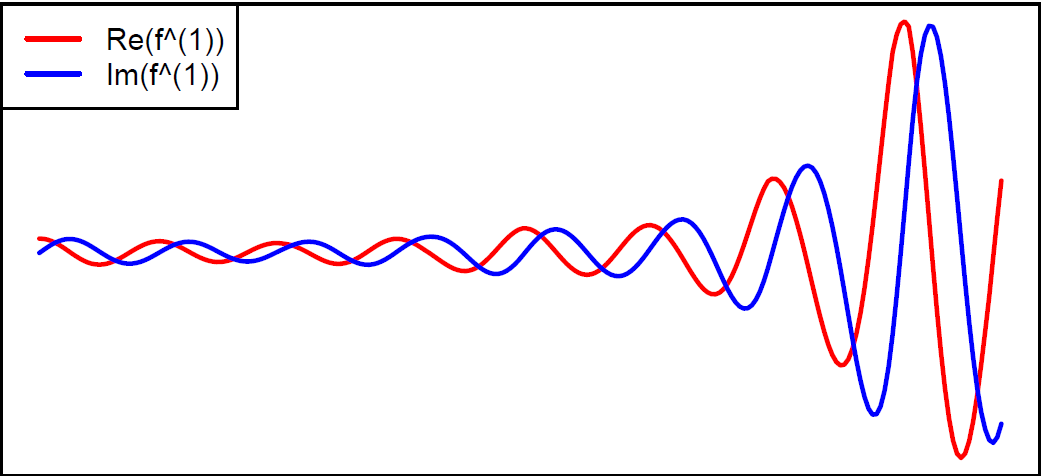
\includegraphics[, height = 3cm]{f1.PNG}
        \caption{Графики $\Re(f^{(1)})$ и $\Im(f^{(1)})$.}
    \end{center}
\end{figure}
    
    Видно, что $\Re(f^{(1)})$ $\approx$ $\Im(f^{(1)})$. Тогда как $f^{(1)*}_{\Im} = 0$, а $f^{(1)*}_{\Re} \neq 0$.\\
    \vspace{1em}
    \alert{Вывод:} Результат теоремы не выполняется для общего случая комплексной экспоненты.
\end{frame}

\begin{frame}{Что было сделано}
    \begin{itemize}
        \item Робастные версии SSA были обобщены на комплексный случай.
        \item Комплексные робастные версии SSA были реализованы на R.
        \item Теорема, о выражении первого члена ошибки восстановления метода CSSA через ошибку метода SSA, была сформулирована и доказана .
        \item Аналогичное утверждение для дисперсий первого члена ошибки восстановления было сформулировано и доказано.
        \item Аналитическая формула для первого приближения ошибки восстановления, в случае константного комплексного сигнала, возмущённого комплексным выбросом, была получена.  
    \end{itemize}
\end{frame}

\begin{frame}{Что планируется сделать}
    \begin{itemize}
        \item Рассмотреть возможность обобщения теоремы в общем и утверждения утверждения про дисперсии в частности на случай синусоидальных сигналов со сдвигом, не равным $\pi / 2$.
        \item Рассмотреть случай возмущения комплексной экспоненты.
        \item Рассмотреть трудоёмкость представленных робастных методов.
    \end{itemize}
\end{frame}

\end{document}
